\subsection{双电子效率修正}
\label{chap:pair_eff}

因为最后我们是得到的双电子谱,所以在最后进行效率修正的时候我们需要的是双电子对的重建效率。在本分析当中,电子对在二维空间($p_T~-~M_{ee}$平面)上重建效率是通过蒙特卡洛模拟(Monte Carlo Simulation)的方法计算得到的。而对于双电子的来源,我们有两种不同的模拟方法:
\begin{itemize}
    \item[1.]虚光子模拟:在这种方法中由虚光子对作为整个模拟的输入。对于虚光子来说,其动力学性质如下:在强子衰变模拟(将于\ref{ch:cocktail}讨论)当中得到的$p_T$和$M_{ee}$的来作为其$p_T$和$M_{ee}$的输入分布。其方位角$\phi$和快度(rapidity)分布分别为在$-\pi~-~\pi$以及-1 - 1范围内的平的分布。同时在虚光子在整个空间各向同性地衰变为双电子对。
    \item[2.]强子衰变模拟:在这种情况下的双电子分布为来自于已知的各种来源的混合。强子的衰变在模拟时所用的方法和虚光子模拟类似,也是在整个空间各向同性的衰变为双电子对,但是对于来源于重味强子的半轻子衰变的双电子,其由Pythia模拟产生,在这个过程中产生的双电子对是强相关的。
\end{itemize}
单电子的探测效率通过式\ref{eq:single_e}计算得到。对于电子对来说,每一个电子能否被探测器重建出来都是一个独立的事件,所以电子对的重建效率为两个电子探测效率的乘积,即$\epsilon_{pair} = \epsilon_{e^+}~*~\epsilon_{e^-}$。单电子在进行pT smearing之后再组合成电子对,并在添加电子对探测效率的权重修正之后填入$p_T~-~M_{ee}$的二维直方图。在STAR的接收度($p_T^{e} > 0.2~{\rm GeV/c}$, $|Y_{ee} < 1|$ 以及 $|\eta_e| < 1$)内,如式通过计算添加效率权重修正和未添加效率权重两个直方图之间的比值得到在不同区间内的双电子探测效率。图\ref{fig:Compare_PairEff}为\sNN = 54.4 GeV金-金对撞当中不同中心度下的双电子重建效率。

\begin{figure}[htb]
    \begin{center}
    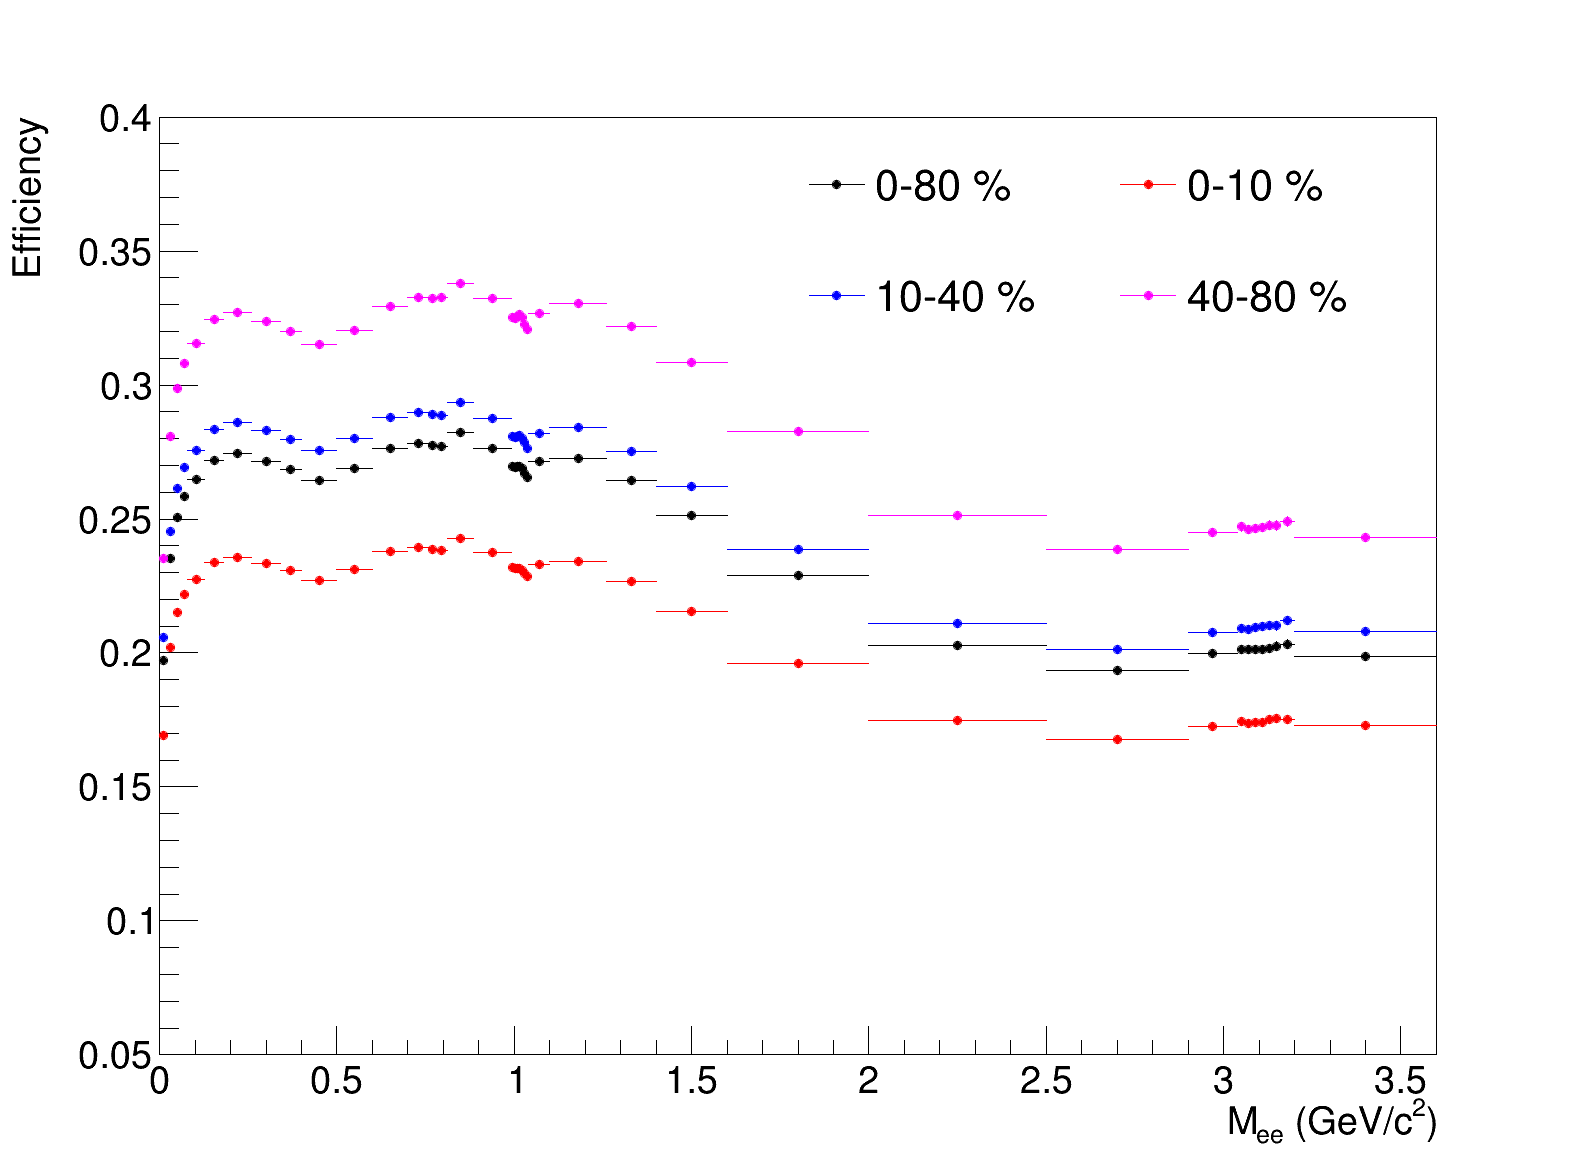
\includegraphics[width=0.75\textwidth,clip]{figures/Chapter4/Compare_PairEff.png}
    \end{center}
    \caption[不同中心度下的双电子重建效率]{\sNN = 54.4 GeV金-金对撞当中不同中心度下的双电子重建效率}
    \label{fig:Compare_PairEff}
\end{figure}

\subsection{接收度修正}
\label{chap:pair_acc}

在上一小节当中我们提到了STAR的接收度,如果我们要将STAR的测量结果和其他实验当中的结果进行比较,我们需要做的是要将STAR的结果修正到全空间当中去,消除STAR接收度的影响。而STAR的接收度修正因子可以通过和双电子效率类似的方式计算得到。计算方法如式\ref{eq:STAR_acc}所示。图\ref{fig:Accep_VP}\sNN = 54.4 GeV金-金对撞当中通过虚光子作为输入计算得到的STAR接受度修正因子。
\begin{equation}
    \label{eq:STAR_acc}
    f_{STAR acc.} = \frac{nPairs(p_T^{e} > 0.2~{\rm GeV/c} \&\& |Y_{ee} < 1| \&\& |\eta_e| < 1)}{nPairs}
\end{equation}
\begin{figure}[htb]
    \begin{center}
    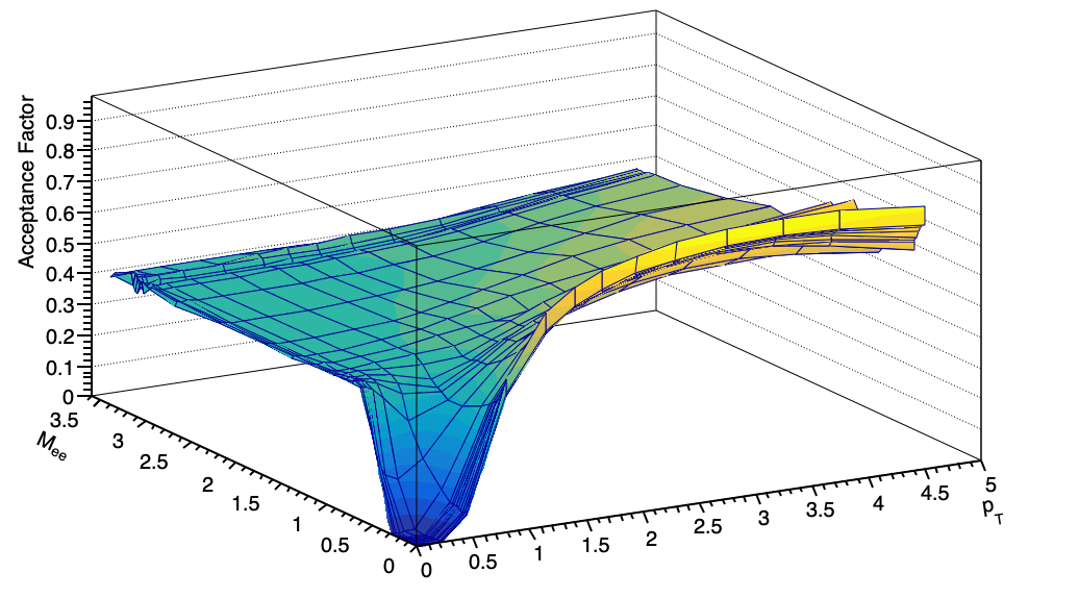
\includegraphics[width=0.75\textwidth,clip]{figures/Chapter4/Accep_VP.png}
    \end{center}
    \caption[通过虚光子作为输入计算得到的STAR接受度修正因子]{\sNN = 54.4 GeV金-金对撞当中通过虚光子作为输入计算得到的STAR接受度修正因子}
    \label{fig:Accep_VP}
\end{figure}
